\documentclass[12pt]{extarticle}
\usepackage[a4paper,margin=1in]{geometry}
\usepackage{amsmath}
\usepackage{graphicx}
\usepackage{float}
\usepackage{subcaption}
\usepackage{fontawesome}
\usepackage[colorlinks=true, linkcolor=blue, urlcolor=blue]{hyperref}

\begin{document}
\begin{titlepage}
    \begin{center}
        
\includegraphics[width=0.3\textwidth]{iitb_logo.png}\\[1.5cm]
        {\LARGE \bfseries Blockchain Arena}\\
        \vspace{0.5cm}
        {\Large \bfseries Simulating Mining Wars and Network Attacks}\\
        \vspace{0.5cm}
        {\Large \bfseries Assignment 1: P2P Network Simulation}\\
        \vspace{1.5cm}
        {\Large \bf Release Date: May 30, 2025}\\
        \vspace{0.5cm}
        {\Large \bf Due Date: 23:59hrs, June 5, 2025}\\
        \vspace{3cm}
        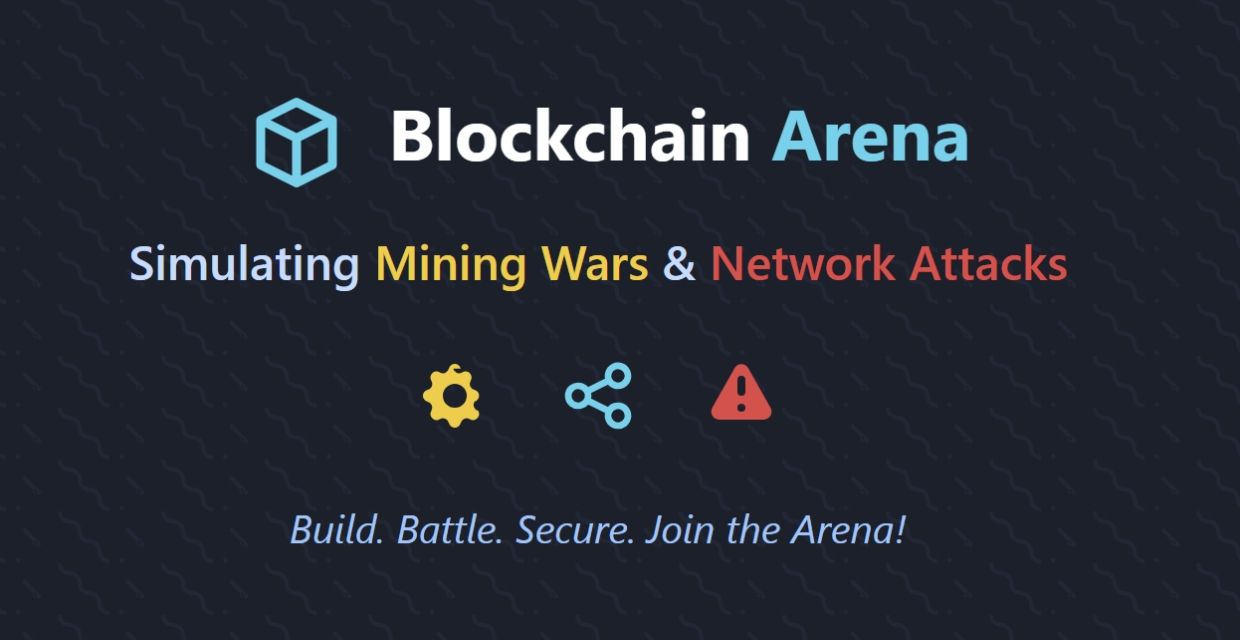
\includegraphics[width=0.9\textwidth]{blockchain_arena.jpeg}\\[1.5cm]
    \end{center}
\end{titlepage}

\section*{Objective}
Welcome to the first assignment for the ``Blockchain Arena" project! This assignment focuses on setting up your development environment and building a foundational Peer-to-Peer (P2P) network. This network will set the stone for building the cryptocurrency network, transaction propagation, and mining.

\section*{Task 1: Setup (Essential)}
\begin{itemize}
    \item \textbf{Git \& GitHub}: Ensure you are familiar with Git and GitHub. If not, learn the basics as they are essential for version control and used widely everywhere.\\Link to the tutorial: \href{https://youtu.be/tRZGeaHPoaw?si=KTOgtqin7e2d0rI8}{Git and GitHub Essentials}.\\ Create a local repository for this project, publish it on GitHub, and either make it public or add me as a collaborator if you want to keep it private (GitHub ID: \texttt{soumitra1854}). Share the repository link.
    \item \textbf{Development Environment}: Set up Python or C++ on your system and verify that all required tools and libraries (e.g., \texttt{NetworkX} for Python) are installed and functional.
\end{itemize}

\section*{Task 2: P2P Network Construction \& Visualization}
I hope all of you have watched the 4th video of CS 765: Introduction to Blockchain and cryptocurrency that I have shared earlier. In this assignment, you will implement a basic P2P network structure that will be used in the later stages of the project.
\subsection*{Problem Statement}
Develop a program to generate and visualize an undirected P2P network.
\subsubsection*{Core Requirements:}
\begin{itemize}
    \item \textbf{Number of Peers}: Choose a random number between 50 to 100.
    \item \textbf{Peer Degree}: Each peer must connect to 3 to 6 other peers ($3 \le \text{deg}(v) \le 6$).
    \item \textbf{Network Connectivity}: The entire graph must be connected (path between any two peers should exist).
    \item \textbf{Validation \& Regeneration}:
          \begin{itemize}
              \item After generation, \textbf{verify} all above conditions.
              \item If invalid (not connected or degree violation), discard and \textbf{recreate the graph from scratch}. Repeat until a valid network is obtained.
              \item Think carefully about how to efficiently check connectivity and degree conditions, and the implementation strategy.
          \end{itemize}
\end{itemize}

\subsection*{Implementation Notes:}
\begin{itemize}
    \item \textbf{Language}: Python or C++.
    \item \textbf{Structure}: A \texttt{Network} class is recommended for managing peers and connections.
    \item \textbf{Connectivity Check}: Use BFS or DFS.
\end{itemize}

\subsection*{Visualization:}
\begin{itemize}
    \item Visualize the valid network clearly showing peers and connections.
    \item \textbf{Python users}: Use \texttt{NetworkX} with \texttt{matplotlib}.
    \item \textbf{C++ users}: Output graph structure (e.g., edge list) to a file; use a Python script with \texttt{NetworkX} to visualize from this file.
    \item Save the image (e.g., \texttt{network.png}) and include it in your submission.
\end{itemize}

\section*{Submission}
\begin{itemize}
    \item Push all source code, visualization image, and a \texttt{README.md} to your GitHub repo.
    \item \texttt{README.md} should include: your name and rollno, brief run instructions, and any critical dependencies.
\end{itemize}

\section*{Quick Tips}
\begin{itemize}
    \item Represent connections efficiently (e.g., adjacency list).
    \item Ensure random connections are undirected and degrees are updated correctly.
    \item Test connectivity algorithms on simple cases.
\end{itemize}

\textbf{Questions? Ask during our online sessions!} Good luck! \faThumbsOUp

\end{document}
